\chapter{Applications of the Integral}
\label{chp:applications_of_the_Integral}			

\section{Volumes of Revolution}

\begin{figure}[h]
\caption{Opening up the Volumes of Revolution tutor using menus.}
\centering
\adjincludegraphics[width=\textwidth,trim={{.3\width} 0 {.1\width} 0},clip]{tutorials/figures/VoRTutorLoad1-eps-converted-to.pdf}
\end{figure}

\begin{figure}[h]
\caption{Opening up the Volumes of Revolution tutor using commands. The \texttt{Student[Calculus1])} package is required.}
\centering
\adjincludegraphics[width=\textwidth,trim={0 {0.1\height} {.5\width} {0.2\height}},clip]{tutorials/figures/VoRTutorLoad2-eps-converted-to.pdf}
\end{figure}

\newpage

\subsection*{Example: Rotating the region bounded by $x^2-4$ and $-x^2+4$ about the line $y=2$}

\begin{figure}
\caption{Plotting the 2D region first is a good practice before revolving around the given axis.}
\centering
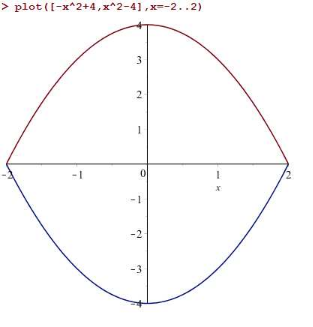
\includegraphics[width=0.6\textwidth]{tutorials/figures/VoRTutorQ0-1-eps-converted-to.pdf}\\
\end{figure}

\begin{figure}
\caption{Setting the Volumes of Revolution tutor to revolve the region about a horizontal axis.}
\centering
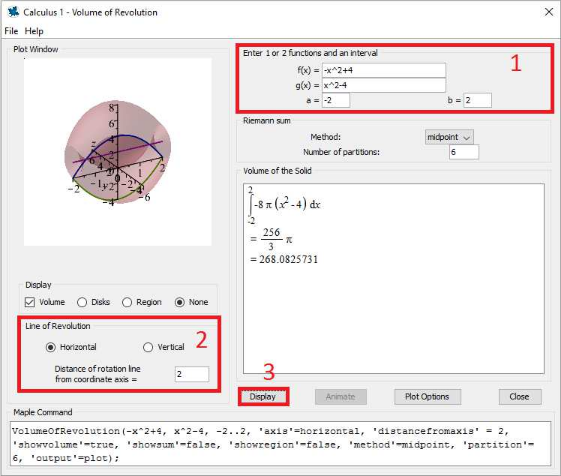
\includegraphics[width=0.9\textwidth]{tutorials/figures/VoRTutorQ1-1-eps-converted-to.pdf}
\end{figure}

\clearpage

\subsection*{Example: Rotating the region bounded by $x^2-4$ and $-x^2+4$ about the line $x=-3$}

\begin{figure}
\caption{Setting the Volumes of Revolution tutor to revolve the region about a vertical axis.}
\centering
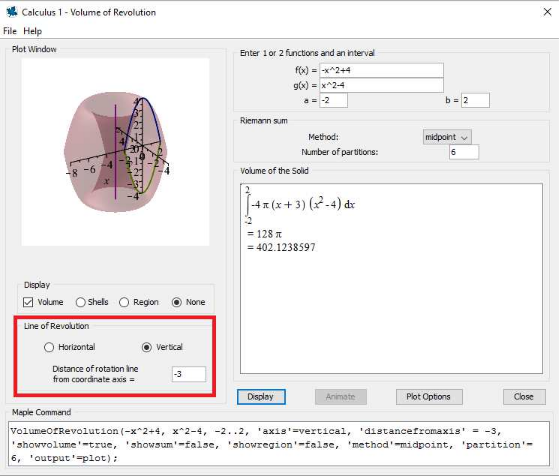
\includegraphics[width=0.9\textwidth]{tutorials/figures/VoRTutorQ1-2-eps-converted-to.pdf}
\end{figure}

\section{Arc Length}
 Suppose we want to find the arc length of the function between two values. We can use the ArcLength command.
\begin{maplegroup}
\begin{mapleinput}
\mapleinline{active}{1d}{with(Student[Calculus1]):
}{}
\end{mapleinput}
\end{maplegroup}

\begin{maplegroup}
\begin{mapleinput}
\mapleinline{active}{1d}{g(x) := x\symbol{94}2;
}{}
\end{mapleinput}
\mapleresult
\begin{maplelatex}
\mapleinline{inert}{2d}{g := proc (x) options operator, arrow; x^2 end proc}{\[\displaystyle g\, := \,x\mapsto {x}^{2}\]}
\end{maplelatex}
\end{maplegroup}

\begin{maplegroup}
\begin{mapleinput}
\mapleinline{active}{1d}{arcg := ArcLength( g(x), x=0..Pi);
}{}
\end{mapleinput}
\mapleresult
\begin{maplelatex}
\mapleinline{inert}{2d}{arcg := (1/2)*Pi*sqrt(4*Pi^2+1)-(1/4)*ln(-2*Pi+sqrt(4*Pi^2+1))}{\[\displaystyle {\it arcg}\, := \,1/2\,\pi \, \sqrt{4\,{\pi }^{2}+1}-1/4\,\ln  \left( -2\,\pi + \sqrt{4\,{\pi }^{2}+1} \right) \]}
\end{maplelatex}
\end{maplegroup}

\begin{maplegroup}
\begin{mapleinput}
\mapleinline{active}{1d}{evalf(arcg);
}{}
\end{mapleinput}
\mapleresult
\begin{maplelatex}
\mapleinline{inert}{2d}{10.62814707}{\[\displaystyle  10.62814707\]}
\end{maplelatex}
\end{maplegroup}

\begin{maplegroup}
\begin{mapleinput}
\mapleinline{active}{1d}{f(x) := sin(x);
}{}
\end{mapleinput}
\mapleresult
\begin{maplelatex}
\mapleinline{inert}{2d}{f := proc (x) options operator, arrow; sin(x) end proc}{\[\displaystyle f\, := \,x\mapsto \sin \left( x \right) \]}
\end{maplelatex}
\end{maplegroup}

\begin{maplegroup}
\begin{mapleinput}
\mapleinline{active}{1d}{arcf := ArcLength( f(x), x=0..Pi);
}{}
\end{mapleinput}
\mapleresult
\begin{maplelatex}
\mapleinline{inert}{2d}{arcf := 2*sqrt(2)*EllipticE((1/2)*sqrt(2))}{\[\displaystyle {\it arcf}\, := \,2\, \sqrt{2}{\it EllipticE} \left( 1/2\, \sqrt{2} \right) \]}
\end{maplelatex}
\end{maplegroup}

\begin{maplegroup}
\begin{mapleinput}
\mapleinline{active}{1d}{evalf(arcf);
}{}
\end{mapleinput}
\mapleresult
\begin{maplelatex}
\mapleinline{inert}{2d}{3.820197788}{\[\displaystyle  3.820197788\]}
\end{maplelatex}
\end{maplegroup}

To show what integral is evaluated for calculating the arclength we change the output to be integral.

\begin{maplegroup}
\begin{mapleinput}
\mapleinline{active}{1d}{ArcLength( f(x), x=0..Pi, output=integral);
}{}
\end{mapleinput}
\mapleresult
\begin{maplelatex}
\mapleinline{inert}{2d}{Int(sqrt(cos(x)^2+1), x = 0 .. Pi)}{\[\displaystyle \int _{0}^{\pi }\! \sqrt{ \left( \cos \left( x \right)  \right) ^{2}+1}{dx}\]}
\end{maplelatex}
\end{maplegroup}